\documentclass{standalone}
\usepackage{tikz}
\usetikzlibrary{shapes.geometric, arrows}

% Configuración de estilos
\tikzset{
  startstop/.style={rectangle, rounded corners, minimum width=3cm, minimum height=1cm, text centered, draw=black, fill=red!30},
  io/.style={trapezium, trapezium left angle=70, trapezium right angle=110, minimum width=3cm, minimum height=1cm, text centered, draw=black, fill=blue!30},
  process/.style={rectangle, minimum width=3cm, minimum height=1cm, text centered, draw=black, fill=orange!30},
  decision/.style={diamond, minimum width=3cm, minimum height=1cm, text centered, draw=black, fill=green!30},
  arrow/.style={thick,->,>=stealth}
}

\begin{document}

    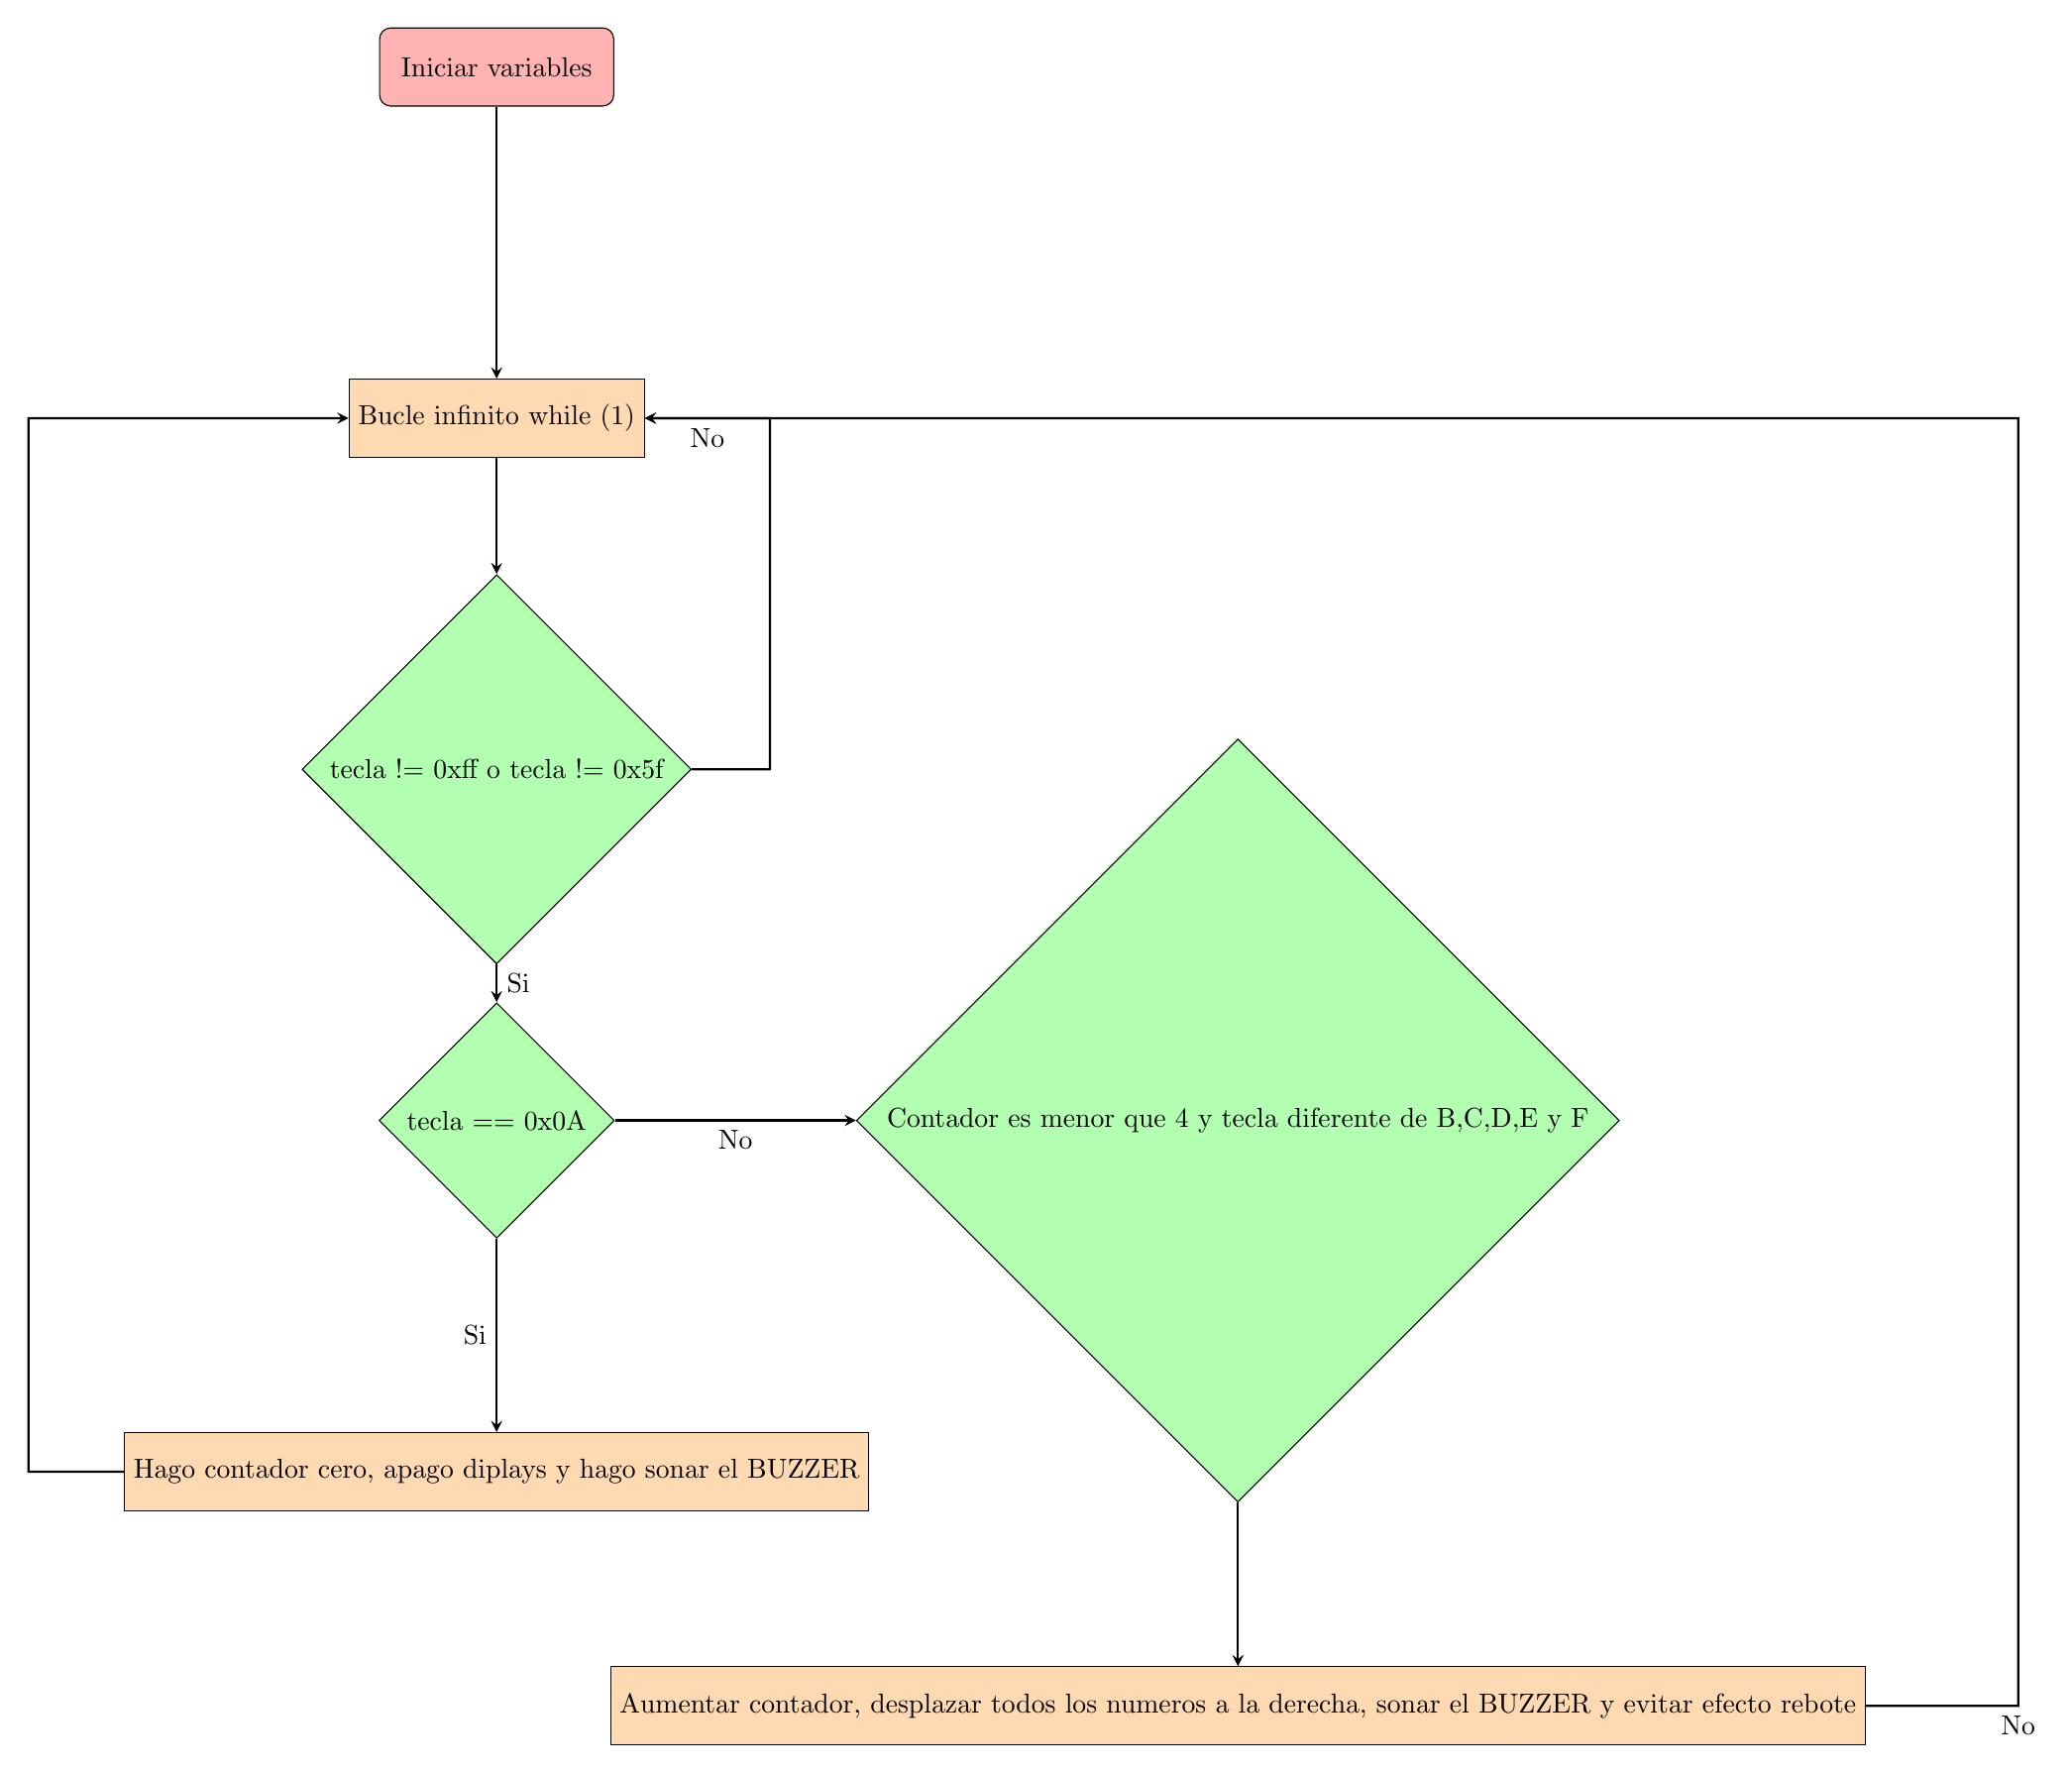
\begin{tikzpicture}[node distance=4.5cm]

        % Bloque 1: Inicialización
        \node (start) [startstop] {Iniciar variables};
        \node (bucle) [process, below of=start] {Bucle infinito while (1)};
        
        % Bloque 2: Verificar tecla
        \node (condicion1) [decision, below of=bucle] {tecla != 0xff o tecla != 0x5f};
        
        % Bloque 3: Verificar tecla "A"
        \node (condicion2) [decision, below of=condicion1] {tecla == 0x0A};
        \node (hacer1) [process, below of = condicion2] {Hago contador cero, apago diplays y hago sonar el BUZZER};
        \node (condicion3)[decision, right of = condicion2,xshift=5cm] {Contador es menor que 4 y tecla diferente de B,C,D,E y F};
        \node (hacer2)[process, below of = condicion3, yshift=-3cm]{Aumentar contador, desplazar todos los numeros a la derecha, sonar el BUZZER y evitar efecto rebote};

        % Flechas
        \draw [arrow] (start) -- (bucle);
        \draw [arrow] (bucle) -- (condicion1);
        \draw [arrow] (condicion1.east) --++ (1,0) --++(0,4.5)-- node[anchor = north]{No} (bucle.east);
        \draw [arrow] (condicion1) --node[anchor=west]{Si} (condicion2);
        \draw [arrow] (condicion2) --node[anchor=east]{Si} (hacer1);
        \draw [arrow] (hacer1) --++(-6,0)--++(0,13.5) --(bucle.west);
        \draw [arrow] (condicion2.east) --node[anchor=north]{No} (condicion3.west);
        \draw [arrow] (condicion3) -- (hacer2);
        \draw [arrow] (hacer2) --++(10,0) node[anchor=north]{No} --++(0,16.5) --(bucle.east);
        \end{tikzpicture}

\end{document}